\documentclass[border=8pt]{standalone}
\usepackage[T1]{fontenc}\usepackage[utf8]{inputenc}
\usepackage{helvet}\renewcommand{\familydefault}{\sfdefault}
\usepackage{tikz,xcolor}
\usetikzlibrary{arrows.meta,positioning,shapes.geometric,shapes.multipart,calc,fit,backgrounds,decorations.markings}
\definecolor{ink}{HTML}{1E1B16}\definecolor{paper}{HTML}{FBF8F2}\definecolor{clay}{HTML}{B5482A}\definecolor{soft}{HTML}{F1E9DA}\definecolor{pine}{HTML}{24402F}
\tikzset{
  every node/.style={font=\small,text=ink},
  >=Stealth, line/.style={draw=ink,line width=0.8pt},
  cls/.style={rectangle split,rectangle split parts=3,draw=ink,line width=0.8pt,fill=soft,align=left,inner xsep=6pt,inner ysep=4pt,
              rectangle split part align={center,left,left},minimum width=3.0cm},
  cls2/.style={rectangle split,rectangle split parts=2,draw=ink,line width=0.8pt,fill=soft,align=left,inner xsep=6pt,inner ysep=4pt,
              rectangle split part align={center,left},minimum width=3.0cm},
  box/.style={rectangle,draw=ink,line width=0.8pt,fill=soft,align=center,inner sep=5pt,minimum height=0.8cm},
  state/.style={rectangle,rounded corners=8pt,draw=ink,line width=0.8pt,fill=soft,align=center,inner sep=6pt,minimum width=2.2cm,minimum height=0.9cm},
  act/.style={rectangle,rounded corners=10pt,draw=ink,line width=0.8pt,fill=soft,align=center,inner sep=5pt,minimum width=2.4cm,minimum height=0.8cm},
  dec/.style={diamond,draw=ink,line width=0.8pt,fill=soft,inner sep=1pt,minimum width=0.9cm,minimum height=0.9cm},
  uc/.style={ellipse,draw=ink,line width=0.8pt,fill=soft,align=center,inner sep=3pt,minimum width=3.2cm,minimum height=1.0cm},
  note/.style={rectangle,draw=ink,line width=0.6pt,fill=yellow!12,align=left,inner sep=4pt,font=\footnotesize},
  lab/.style={font=\footnotesize,fill=paper,inner sep=1.5pt},
  err/.style={},
}
\newcommand{\actor}[3]{% x,y,label
  \draw[line width=0.8pt] (#1,#2+0.55) circle (0.17);
  \draw[line width=0.8pt] (#1,#2+0.38)--(#1,#2-0.15) (#1-0.3,#2+0.22)--(#1+0.3,#2+0.22) (#1,#2-0.15)--(#1-0.25,#2-0.6) (#1,#2-0.15)--(#1+0.25,#2-0.6);
  \node[font=\small] at (#1,#2-0.9) {#3};}
\begin{document}
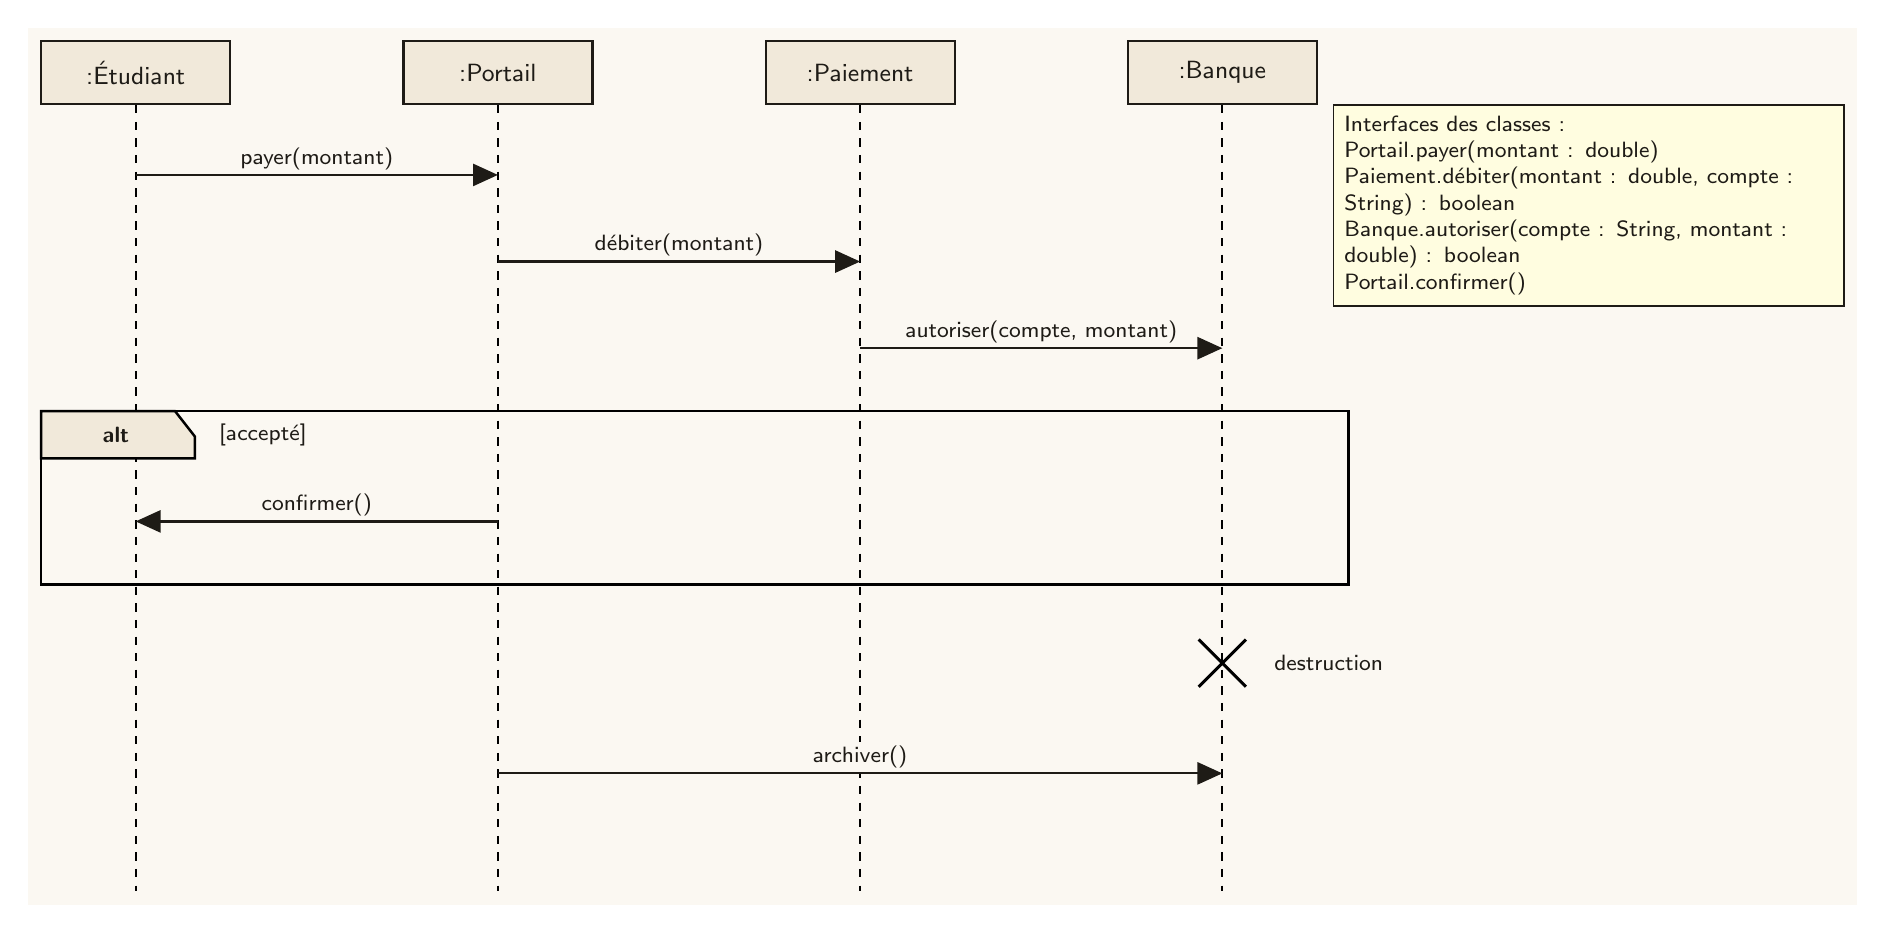
\begin{tikzpicture}[background rectangle/.style={fill=paper},show background rectangle]
\node[box,minimum width=2.4cm] (e) at (0,0) {:Étudiant};
\node[box,minimum width=2.4cm] (p) at (4.6,0) {:Portail};
\node[box,minimum width=2.4cm] (y) at (9.2,0) {:Paiement};
\node[box,minimum width=2.4cm] (k) at (13.8,0) {:Banque};
\draw[dashed,line width=0.7pt] (e.south)--(e.south |- 0,-10.4);
\draw[dashed,line width=0.7pt] (p.south)--(p.south |- 0,-10.4);
\draw[dashed,line width=0.7pt] (y.south)--(y.south |- 0,-10.4);
\draw[dashed,line width=0.7pt] (k.south)--(k.south |- 0,-10.4);
\draw[line,-{Triangle[length=9pt,width=8pt]}] (0,-1.3)--(4.6,-1.3) node[midway,above,lab]{payer(montant)};
\draw[line,-{Triangle[length=9pt,width=8pt]}] (4.6,-2.4)--(9.2,-2.4) node[midway,above,lab]{débiter(montant)};
\draw[line,-{Triangle[length=9pt,width=8pt]}] (9.2,-3.5)--(13.8,-3.5) node[midway,above,lab]{autoriser(compte, montant)};
\draw[line width=0.9pt] (-1.2,-4.3) rectangle (15.4,-6.5);
\draw[line width=0.9pt,fill=soft] (-1.2,-4.3)--(0.5,-4.3)--(0.75,-4.62)--(0.75,-4.9)--(-1.2,-4.9)--cycle;\node[font=\footnotesize\bfseries] at (-0.25,-4.6) {alt};
\node[lab,anchor=west] at (1.0,-4.6) {[accepté]};
\draw[line,-{Triangle[length=9pt,width=8pt]}] (4.6,-5.7)--(0,-5.7) node[midway,above,lab]{confirmer()};
\draw[line width=1.1pt] (13.5,-7.2)--(14.1,-7.8)(13.5,-7.8)--(14.1,-7.2);
\node[lab,anchor=west] at (14.4,-7.5) {destruction};
\draw[line,-{Triangle[length=9pt,width=8pt]}] (4.6,-8.9)--(13.8,-8.9) node[midway,above,lab]{archiver()};
\node[note,anchor=north west,text width=6.2cm] at (15.2,-0.4) {Interfaces des classes :\\ Portail.payer(montant : double)\\ Paiement.débiter(montant : double, compte : String) : boolean\\ Banque.autoriser(compte : String, montant : double) : boolean\\ Portail.confirmer()};
\end{tikzpicture}
\end{document}
